\section{Gestión avanzada}
\label{sec:gestion-avanzada}

El \CMS se gestiona a través de una interfaz web en modo de \emph{portal cautivo} que se activa cuando se accede al modo de gestión tanto del \MI como del \ME.
Ambos módulos proporcionan portales de gestión con la misma estructura y funcionalidad: la única diferencia entre ellos se encuentra en los parámetros de funcionamiento que se pueden configurar.

A continuación se detallan los pasos a seguir para acceder al modo de gestión, así como las diferentes funciones y opciones que se proporcionan.

\subsection{Acceso a la interfaz de gestión}
\label{sec:acceso-gestion}

Como se introduce en la sección~\ref{sec:inicio-rapido} (\textit{\nameref{sec:inicio-rapido}}), el modo de acceso a la interfaz de gestión es el mismo en ambos casos: presionar el único botón independiente que presentan los módulos a la vez se encienden o se reinician.

Para activar la interfaz de gestion del \MIE se hace uso del botón multifunción \circled{I8}:

\begin{enumeratecompact}

\item Mientras pulsa el botón multifunción \circled{I8}, conecte la alimentación USB \circled{I6} del \MI. Si la alimentación ya está conectada, alternativamente, puede presionar el botón de reinicio \circled{I5} mientras pulsa el botón multifunción \circled{I8}. Cuando la luz de notificación de configuración \circled{I3} se encienda de forma fija y en la pantalla LCD \circled{I1} aparezca el texto \emph{Conecta a Config.~Interior} (figura~\ref{fig:screen-config}), suelte el botón \circled{I8}.

\begin{figure}[!b]
  \centering
  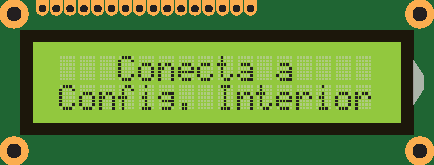
\includegraphics[width=0.6\columnwidth]{images/screen-config}
  \caption{Pantalla del módulo interior: modo gestión}
  \label{fig:screen-config}
\end{figure}


Si el mensaje \emph{Conecta a Config.~Interior} no aparece en la pantalla LCD, comience de nuevo.

\item Con la ayuda de un dispositivo móvil o un ordenador con conexión wifi, busque las redes wifi disponibles y conecte a la red llamada \emph{Config.~Interior} (figura~\ref{fig:interior-select-wifi}, página~\pageref{fig:interior-select-wifi}).

\item En caso de que su dispositivo no le rediriga automáticamente a la página de configuración del \MI, despliegue el área de notificaciones de su dispositivo y pulse la opción \emph{Iniciar sesión en red Wi-Fi ``Config.~Interior''} (figura~\ref{fig:interior-captive-portal-notification}, página~\pageref{fig:interior-captive-portal-notification}).

\item El menú mostrado en la figura~\ref{fig:interior-menu} aparecerá en su pantalla.

\end{enumeratecompact}

En el caso del \MEE, la activación de la interfaz de gestión se realiza mediante el botón de configuración \circled{E4}:

\begin{enumeratecompact}

\item Asegúrese de que el \ME está apagado (interruptor de encendido \circled{E2} en posición \off).

\item Mientras pulsa el botón de configuración \circled{E5} con ayuda de alguna herramienta de punta estrecha y alargada, conecte el \ME moviendo el interruptor de encendido \circled{E2} a la  posición \on.

\item Con la ayuda de un dispositivo móvil o un ordenador con conexión wifi, busque las redes wifi disponibles y conecte a la red llamada \emph{Config.~Exterior} (figura~\ref{fig:exterior-select-wifi}).

\item En caso de que su dispositivo no le rediriga automáticamente a la página de configuración del \ME, despliegue el área de notificaciones de su dispositivo y pulse la opción \emph{Iniciar sesión en red Wi-Fi ``Config.~Exterior''} (figura~\ref{fig:exterior-captive-portal-notification}).

\item El menú mostrado en la figura~\ref{fig:exterior-menu} aparecerá en su pantalla.

\end{enumeratecompact}

\subsection{Opciones de gestión}

La figura~\ref{fig:menu} muestra las opciones de gestión que ofrecen ambos módulos:

\begin{descriptioncompact}

\item[Configurar] --- Permite establecer diversos parámetros de funcionamiento, como nombre del host, frecuencia de actualizaciones, horario de silencion, \etc Las opciones de configuración se describen en la sección~\ref{sec:config}.

\item[Actualizar] --- Permite actualizar el firmware de los distintos módulos sin necesidad de conectarlos físicamente a un ordenador mediante una conexión USB. Las opciones de configuración se describen en la sección~\ref{sec:actualizar}.

\item[Información] --- Muestra información básica del sistema y el hardware de los módulos. Las opciones de configuración se describen en la sección~\ref{sec:info}.

\item[Reiniciar] --- Reinicia el sistema sin guardar los cambios. Las opciones de configuración se describen en la sección~\ref{sec:reinicio}.

\end{descriptioncompact}

\subsubsection{Parámetros de configuración}
\label{sec:config}

\subsubsection{Actualización remota}
\label{sec:actualizar}

\attbegin{Conexión de datos}
Para poder acceder a la interfaz de gestión desde un navegador web ---como \textit{Google Chrome}--- desde su dispositivo móvil, es probable que deba desactivar previamente su conexión de datos.
\attend

\subsubsection{Información}
\label{sec:info}

\subsubsection{Reinicio}
\label{sec:reinicio}

\begin{figure}
\begin{subfigure}{0.49\columnwidth}
  \centering
  \includegraphics[width=1\columnwidth,frame]{images/interior-select-wifi}
  \caption{}
  \label{fig:interior-select-wifi}
\end{subfigure}
\hfill
\begin{subfigure}{0.49\columnwidth}
  \centering
  \includegraphics[width=1\columnwidth,frame]{images/exterior-select-wifi}
  \caption{}
  \label{fig:exterior-select-wifi}
\end{subfigure}
\caption{Conectar a las redes \textit{Config.~Interior} (a) y \textit{Config.~Exterior} (b)}
\end{figure}

\begin{figure}
\begin{subfigure}{0.49\columnwidth}
  \centering
  \includegraphics[width=1\columnwidth,frame]{images/interior-captive-portal-notification}
  \caption{}
  \label{fig:interior-captive-portal-notification}
\end{subfigure}
\hfill
\begin{subfigure}{0.49\columnwidth}
  \centering
  \includegraphics[width=1\columnwidth,frame]{images/exterior-captive-portal-notification}
  \caption{}
  \label{fig:exterior-captive-portal-notification}
\end{subfigure}
\caption{Iniciar sesión en las redes \textit{Config.~Interior} (a) y \textit{Config.~Exterior} (b)}
\end{figure}


\begin{figure}
\begin{subfigure}{0.49\columnwidth}
  \centering
  \includegraphics[width=1\columnwidth,frame]{images/interior-menu}
  \caption{}
  \label{fig:interior-menu}
\end{subfigure}
\hfill
\begin{subfigure}{0.49\columnwidth}
  \centering
  \includegraphics[width=1\columnwidth,frame]{images/exterior-menu}
  \caption{}
  \label{fig:exterior-menu}
\end{subfigure}
\caption{Menú de gestión de los módulos interior (a) y exterior (b)}
\label{fig:menu}
\end{figure}

\begin{figure}
\begin{subfigure}{0.49\columnwidth}
  \centering
  \includegraphics[height=0.94\textheight,frame]{images/interior-config}
  \caption{}
  \label{fig:interior-config}
\end{subfigure}
\hfill
\begin{subfigure}{0.49\columnwidth}
  \centering
  \includegraphics[width=0.9\columnwidth,frame]{images/exterior-config}
  \caption{}
  \label{fig:exterior-config}
\end{subfigure}
\caption{Configuración de los módulos interior (a) y exterior (b)}
\end{figure}

\begin{figure}
\begin{subfigure}{0.49\columnwidth}
  \centering
  \includegraphics[width=1\columnwidth,frame]{images/interior-config-saved}
  \caption{}
  \label{fig:interior-config-saved}
\end{subfigure}
\hfill
\begin{subfigure}{0.49\columnwidth}
  \centering
  \includegraphics[width=1\columnwidth,frame]{images/exterior-config-saved}
  \caption{}
  \label{fig:exterior-config-saved}
\end{subfigure}
\caption{Mensaje de confirmación de configuración guardada en los módulos interior (a) y exterior (b)}
\end{figure}



\begin{figure}
\begin{subfigure}{0.49\columnwidth}
  \centering
  \includegraphics[width=1\columnwidth,frame]{images/interior-firmware-update}
  \caption{}
  \label{fig:interior-firmware-update}
\end{subfigure}
\hfill
\begin{subfigure}{0.49\columnwidth}
  \centering
  \includegraphics[width=1\columnwidth,frame]{images/exterior-firmware-update}
  \caption{}
  \label{fig:exterior-firmware-update}
\end{subfigure}
\caption{Actualización del firmware de los módulos interior (a) y exterior (b)}
\end{figure}

\begin{figure}
\begin{subfigure}{0.32\columnwidth}
  \centering
  \includegraphics[width=1\columnwidth,frame]{images/interior-firmware-update-selection}
  \caption{}
  \label{fig:interior-firmware-update-selection}
\end{subfigure}
\hfill
\begin{subfigure}{0.32\columnwidth}
  \centering
  \includegraphics[width=1\columnwidth,frame]{images/interior-firmware-update-chrome}
  \caption{}
  \label{fig:interior-firmware-update-chrome}
\end{subfigure}
\hfill
\begin{subfigure}{0.32\columnwidth}
  \centering
  \includegraphics[width=1\columnwidth,frame]{images/interior-firmware-update-done}
  \caption{}
  \label{fig:interior-firmware-update-done}
\end{subfigure}
\caption{Actualización del firmware: (a) acceder desde el navegador, (b) seleccionar el fichero .bin, (c) confirmación de actualización correcta}
\end{figure}

\begin{figure}
\begin{subfigure}{0.49\columnwidth}
  \centering
  \includegraphics[width=1\columnwidth,frame]{images/interior-info}
  \caption{}
  \label{fig:interior-info}
\end{subfigure}
\hfill
\begin{subfigure}{0.49\columnwidth}
  \centering
  \includegraphics[width=1\columnwidth,frame]{images/exterior-info}
  \caption{}
  \label{fig:exterior-info}
\end{subfigure}
\caption{Información de los módulos interior (a) y exterior (b)}
\end{figure}

\begin{figure}
\begin{subfigure}{0.49\columnwidth}
  \centering
  \includegraphics[width=1\columnwidth,frame]{images/interior-restart}
  \caption{}
  \label{fig:interior-restart}
\end{subfigure}
\hfill
\begin{subfigure}{0.49\columnwidth}
  \centering
  \includegraphics[width=1\columnwidth,frame]{images/exterior-restart}
  \caption{}
  \label{fig:exterior-restart}
\end{subfigure}
\caption{Reiniciando los módulos interior (a) y exterior (b)}
\end{figure}

